\documentclass{article}
\usepackage{amsmath}
\usepackage[mathletters]{ucs}
\usepackage[utf8x]{inputenc}
\usepackage[margin=1.5in]{geometry}
\usepackage{enumerate}
\newtheorem{theorem}{Theorem}
\usepackage[dvipsnames]{xcolor}
\usepackage{pgfplots}
\setlength{\parindent}{0cm}
\usepackage{graphics}
\usepackage{graphicx} % Required for including images
\usepackage{subcaption}
\usepackage{bigintcalc}
\usepackage{pythonhighlight} %for pythonkode \begin{python}   \end{python}
\usepackage{appendix}
\usepackage{arydshln}
\usepackage{physics}
\usepackage{tikz-cd}
\usepackage{booktabs} 
\usepackage{adjustbox}
\usepackage{mdframed}
\usepackage{relsize}
\usepackage{physics}
\usepackage[thinc]{esdiff}
\usepackage{fixltx2e}
\usepackage{esint}  %for lukket-linje-integral
\usepackage{xfrac} %for sfrac
\usepackage{hyperref} %for linker, må ha med hypersetup
\usepackage[noabbrev, nameinlink]{cleveref} % to be loaded after hyperref
\usepackage{amssymb} %\mathbb{R} for reelle tall, \mathcal{B} for "matte"-font
\usepackage{listings} %for kode/lstlisting
\usepackage{verbatim}
\usepackage{graphicx,wrapfig,lipsum,caption} %for wrapping av bilder
\usepackage{mathtools} %for \abs{x}
\usepackage[norsk]{babel}
\definecolor{codegreen}{rgb}{0,0.6,0}
\definecolor{codegray}{rgb}{0.5,0.5,0.5}
\definecolor{codepurple}{rgb}{0.58,0,0.82}
\definecolor{backcolour}{rgb}{0.95,0.95,0.92}
\pagecolor[rgb]{0.075,0.075,0.075} \color[rgb]{1,1,1} %TODO: Slett når ferdig%
% \lstdefinestyle{mystyle}{
%     backgroundcolor=\color{backcolour},   
%     commentstyle=\color{codegreen},
%     keywordstyle=\color{magenta},
%     numberstyle=\tiny\color{codegray},
%     stringstyle=\color{codepurple},
%     basicstyle=\ttfamily\footnotesize,
%     breakatwhitespace=false,         
%     breaklines=true,                 
%     captionpos=b,                    
%     keepspaces=true,                 
%     numbers=left,                    
%     numbersep=5pt,                  
%     showspaces=false,                
%     showstringspaces=false,
%     showtabs=false,                  
%     tabsize=2
% }

% \lstset{style=mystyle}
\author{Oskar Idland}
\title{FYS2130 - Oblig 2}
\date{}
\begin{document}
\maketitle
\newpage

\section*{Oppgave 1}
\begin{enumerate}[a)]
\item 
Q-faktor er gitt ved
\[
Q = \frac{f_0}{Δf}
\]  
hvor $f_0$ er resonansfrekvensen og $Δf$ er halv-bredden. 
\[
Q = \frac{675 \text{ kHz}}{9 \text{ kHz}} = 75
\]

\subsection*{Oppgave 2}
\begin{figure}[h!]
  \centering
  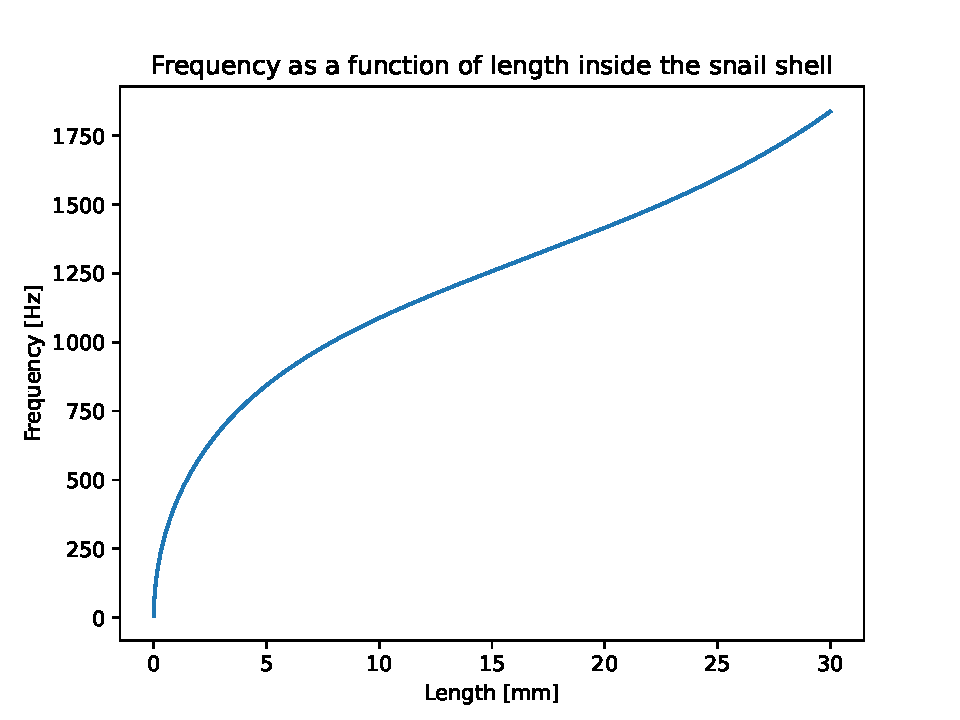
\includegraphics[scale = .45]{figs/1.b.pdf}
  \caption{Plot av frekvens, $f$ som den endrer seg i øret}
  \label{fig: 1.b}
\end{figure}

\begin{figure}[h!]
  \centering
  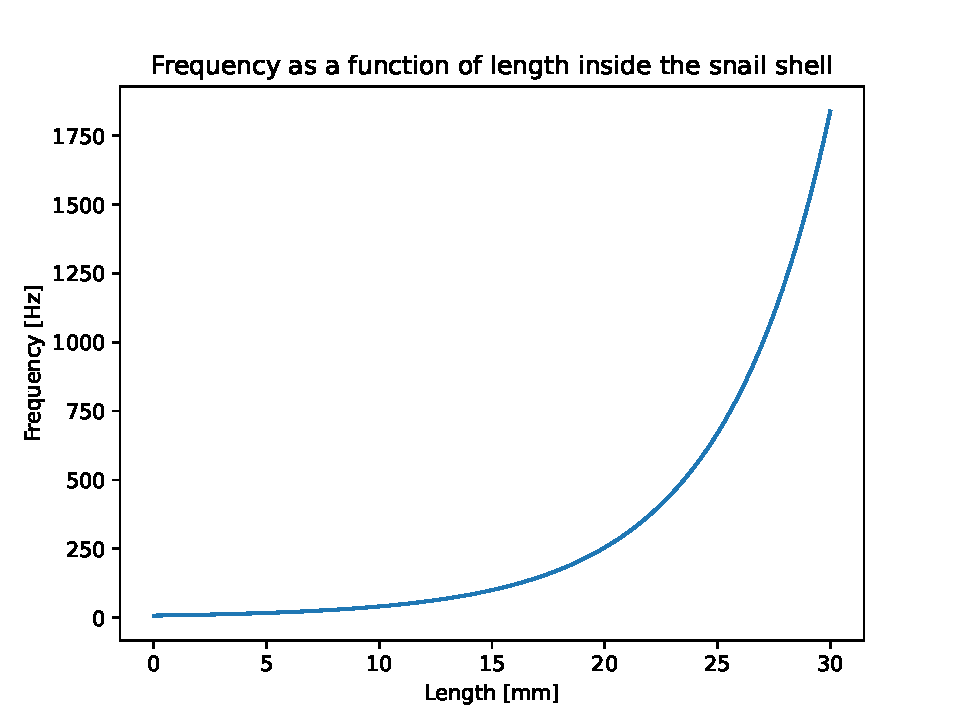
\includegraphics[scale = .45]{figs/1.b_ln.pdf}
  \caption{Plot av frekvens, $f$ som den endrer seg i øret, me}
  \label{fig:figure1}
\end{figure}
Vi ser at med en logaritmisk fjærstivhet får vi en veldig annerledes frekvens avhengig av posisjon. Den lineære varianten har ikke noe overlapp med seg selv.
\item
\begin{figure}[h!]
  \centering
  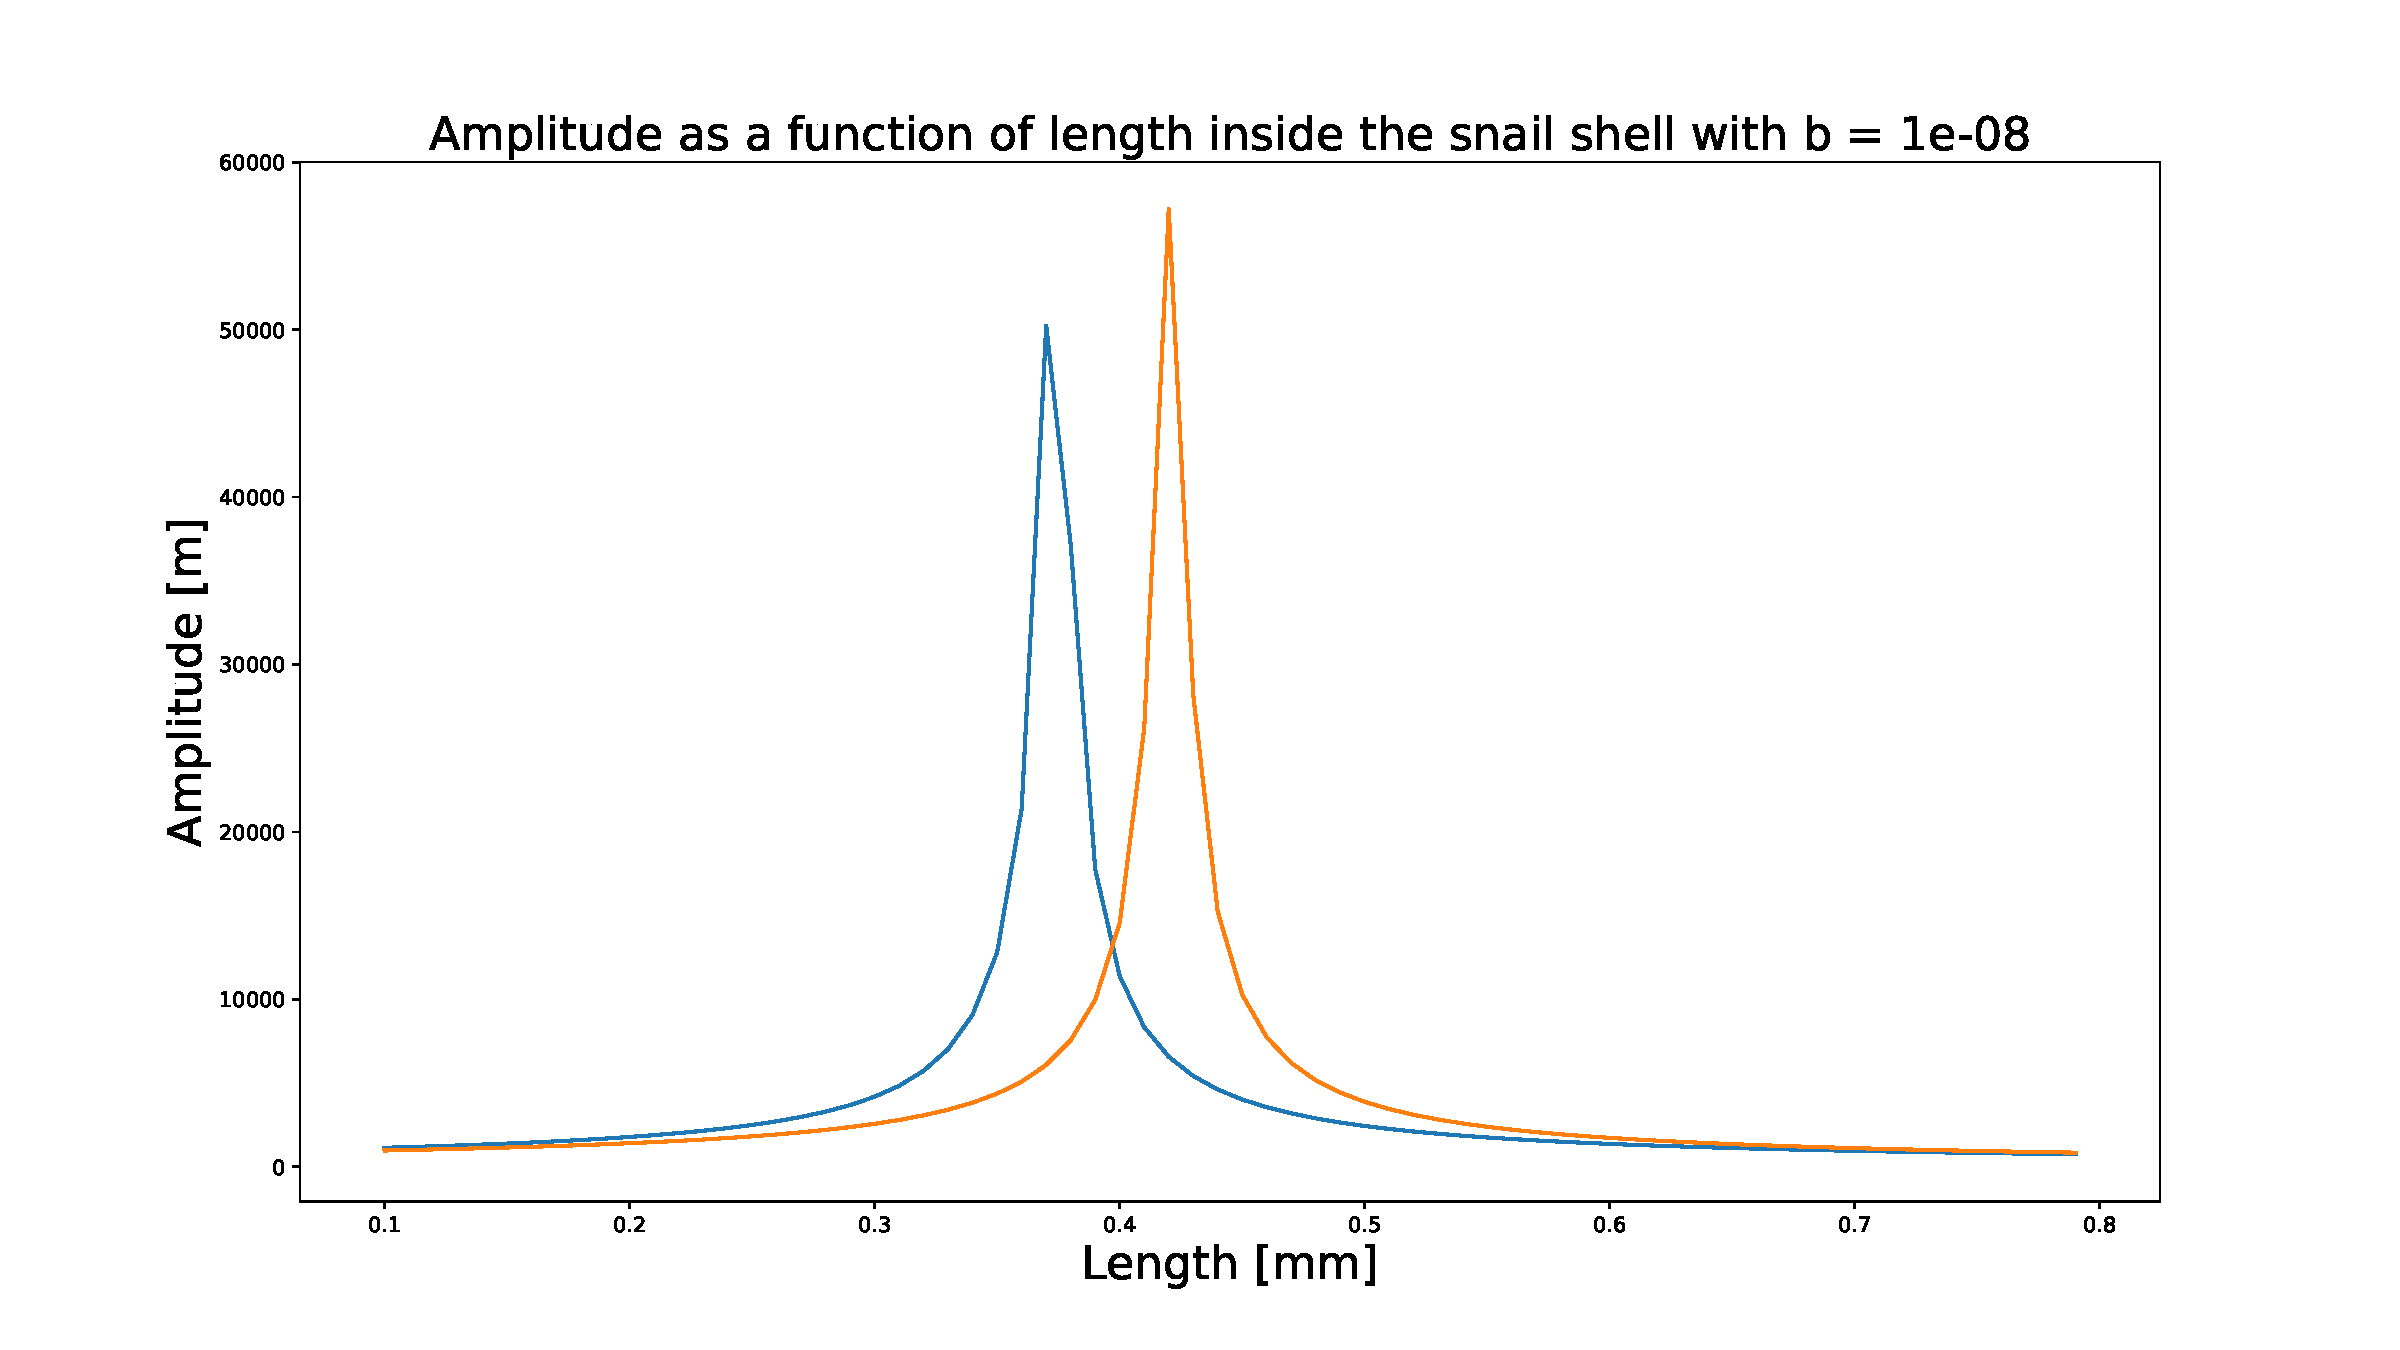
\includegraphics[width = \textwidth]{figs/2.b.pdf}
  \caption{Øret klarer å skille mellom frekvensene $C_4$ og $C_4^{♯}$ med dempningsfaktor $b = 1E-8$}
  \label{fig: 2.b}
\end{figure}
\item
Vi bruker at Q er gitt ved 
\[
Q = \sqrt{\frac{mk}{b^2}}
\]

\begin{figure}[h!]
  \centering
  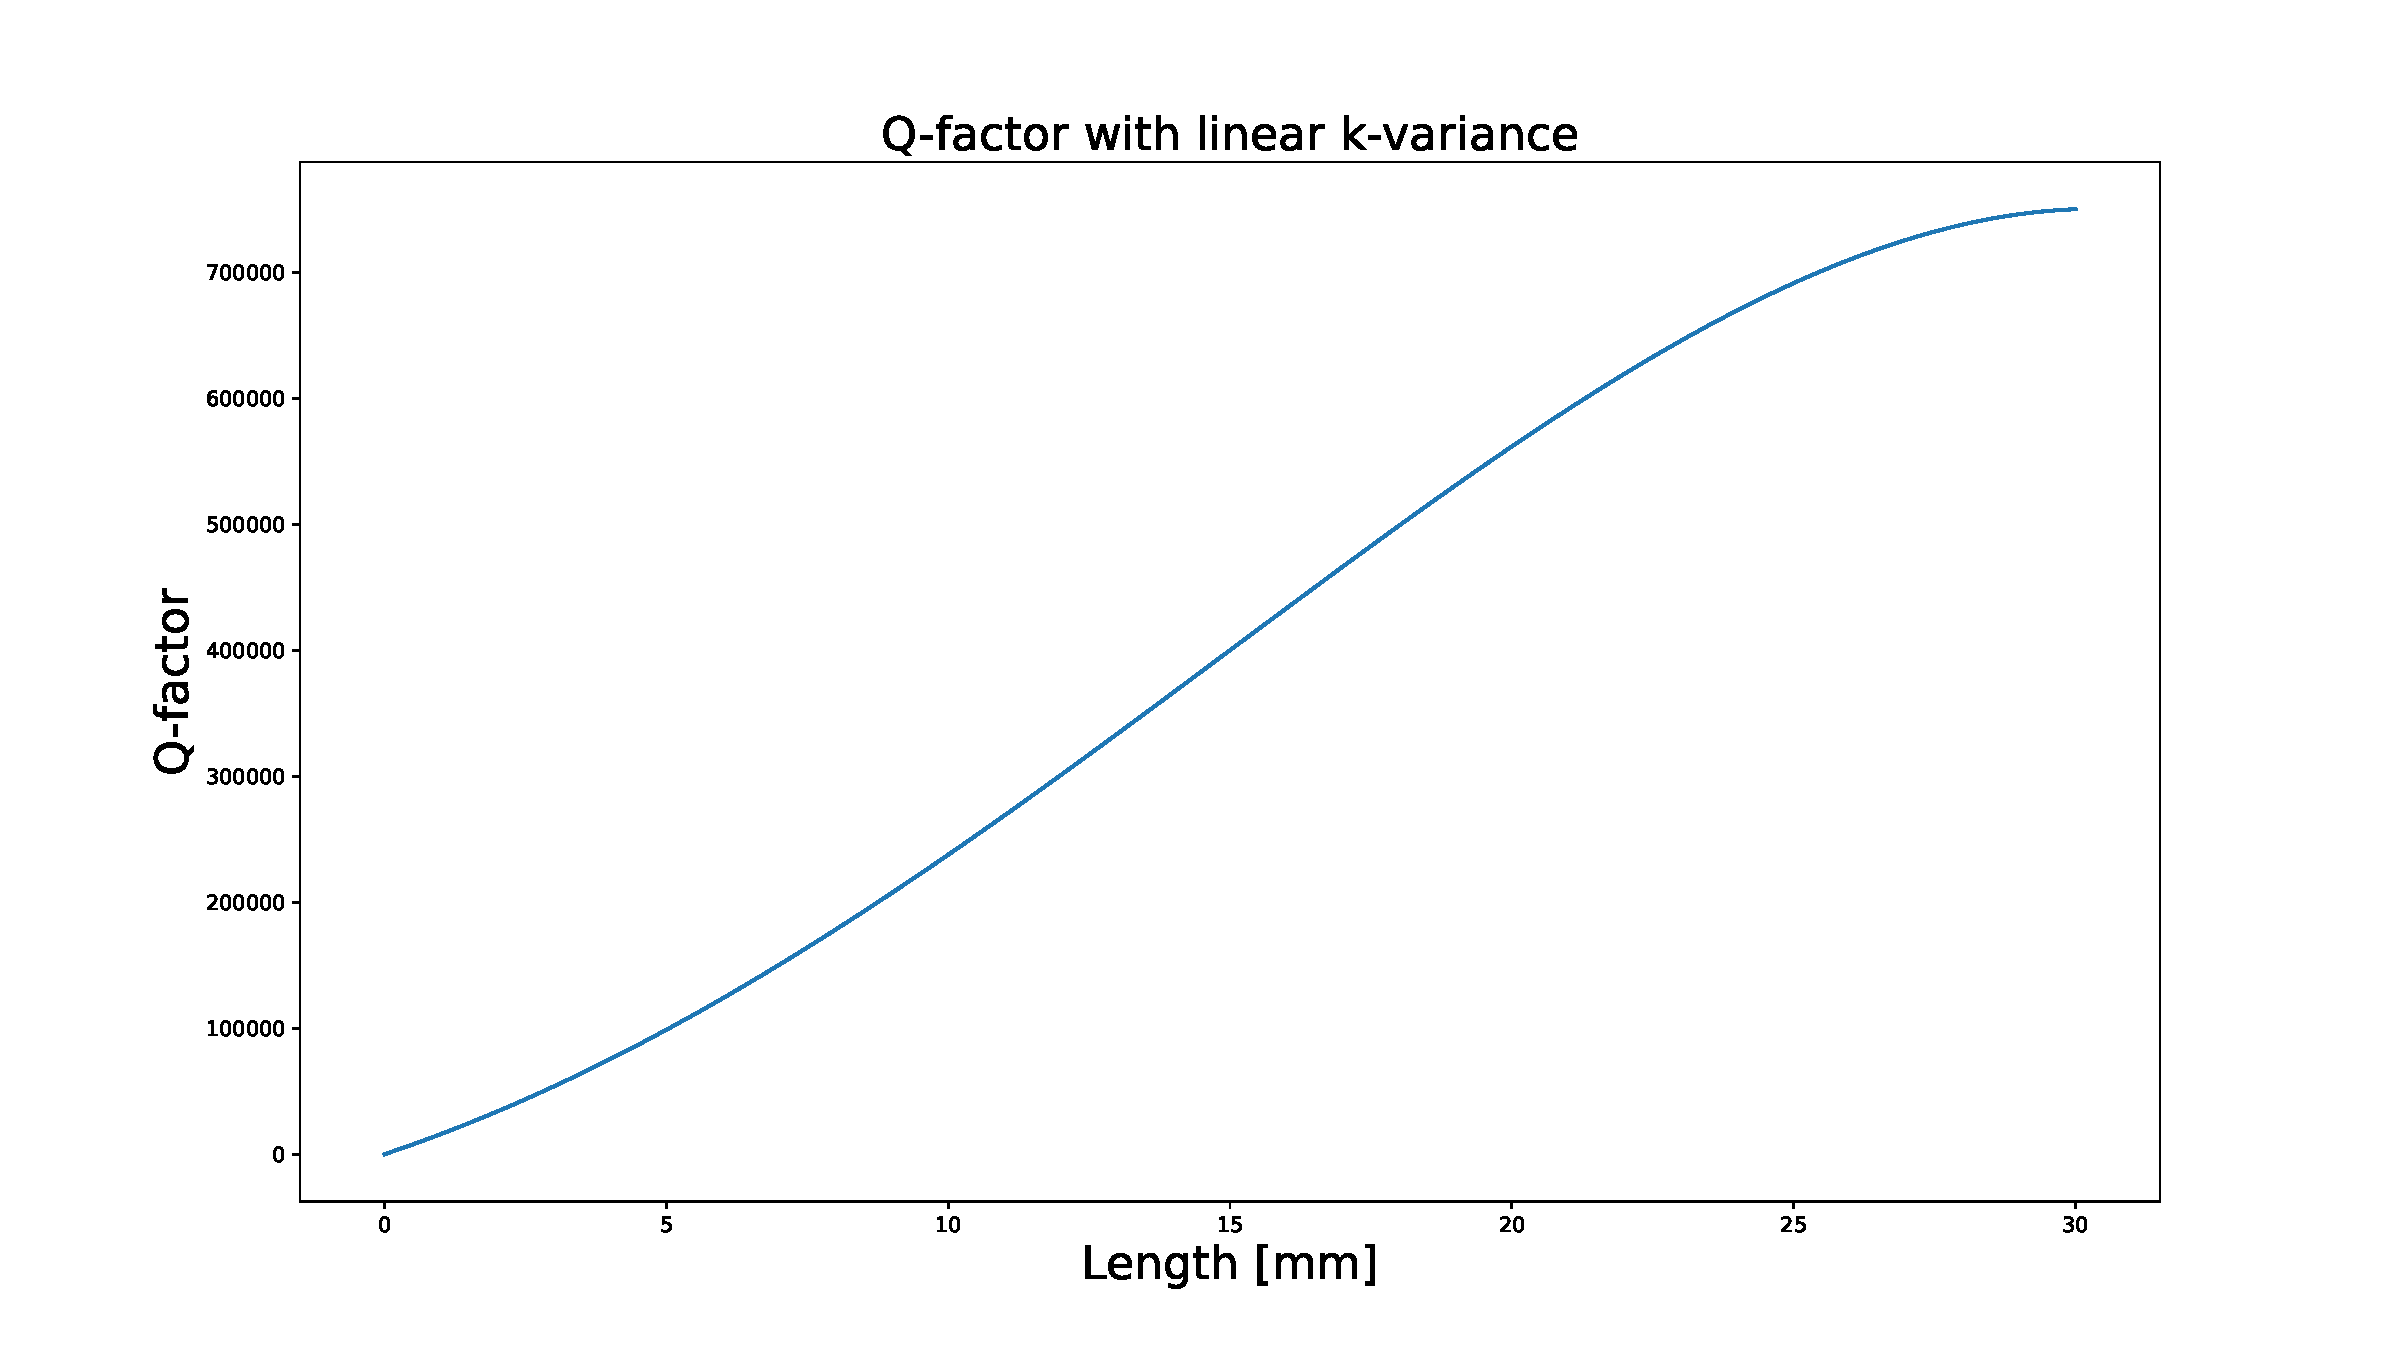
\includegraphics[width = \textwidth]{figs/2.c.pdf}
  \caption{Plot av Q-faktor}
  \label{fig: 2.c}
\end{figure}


\newpage
\begin{figure}[h!]
  \item 
  \centering
  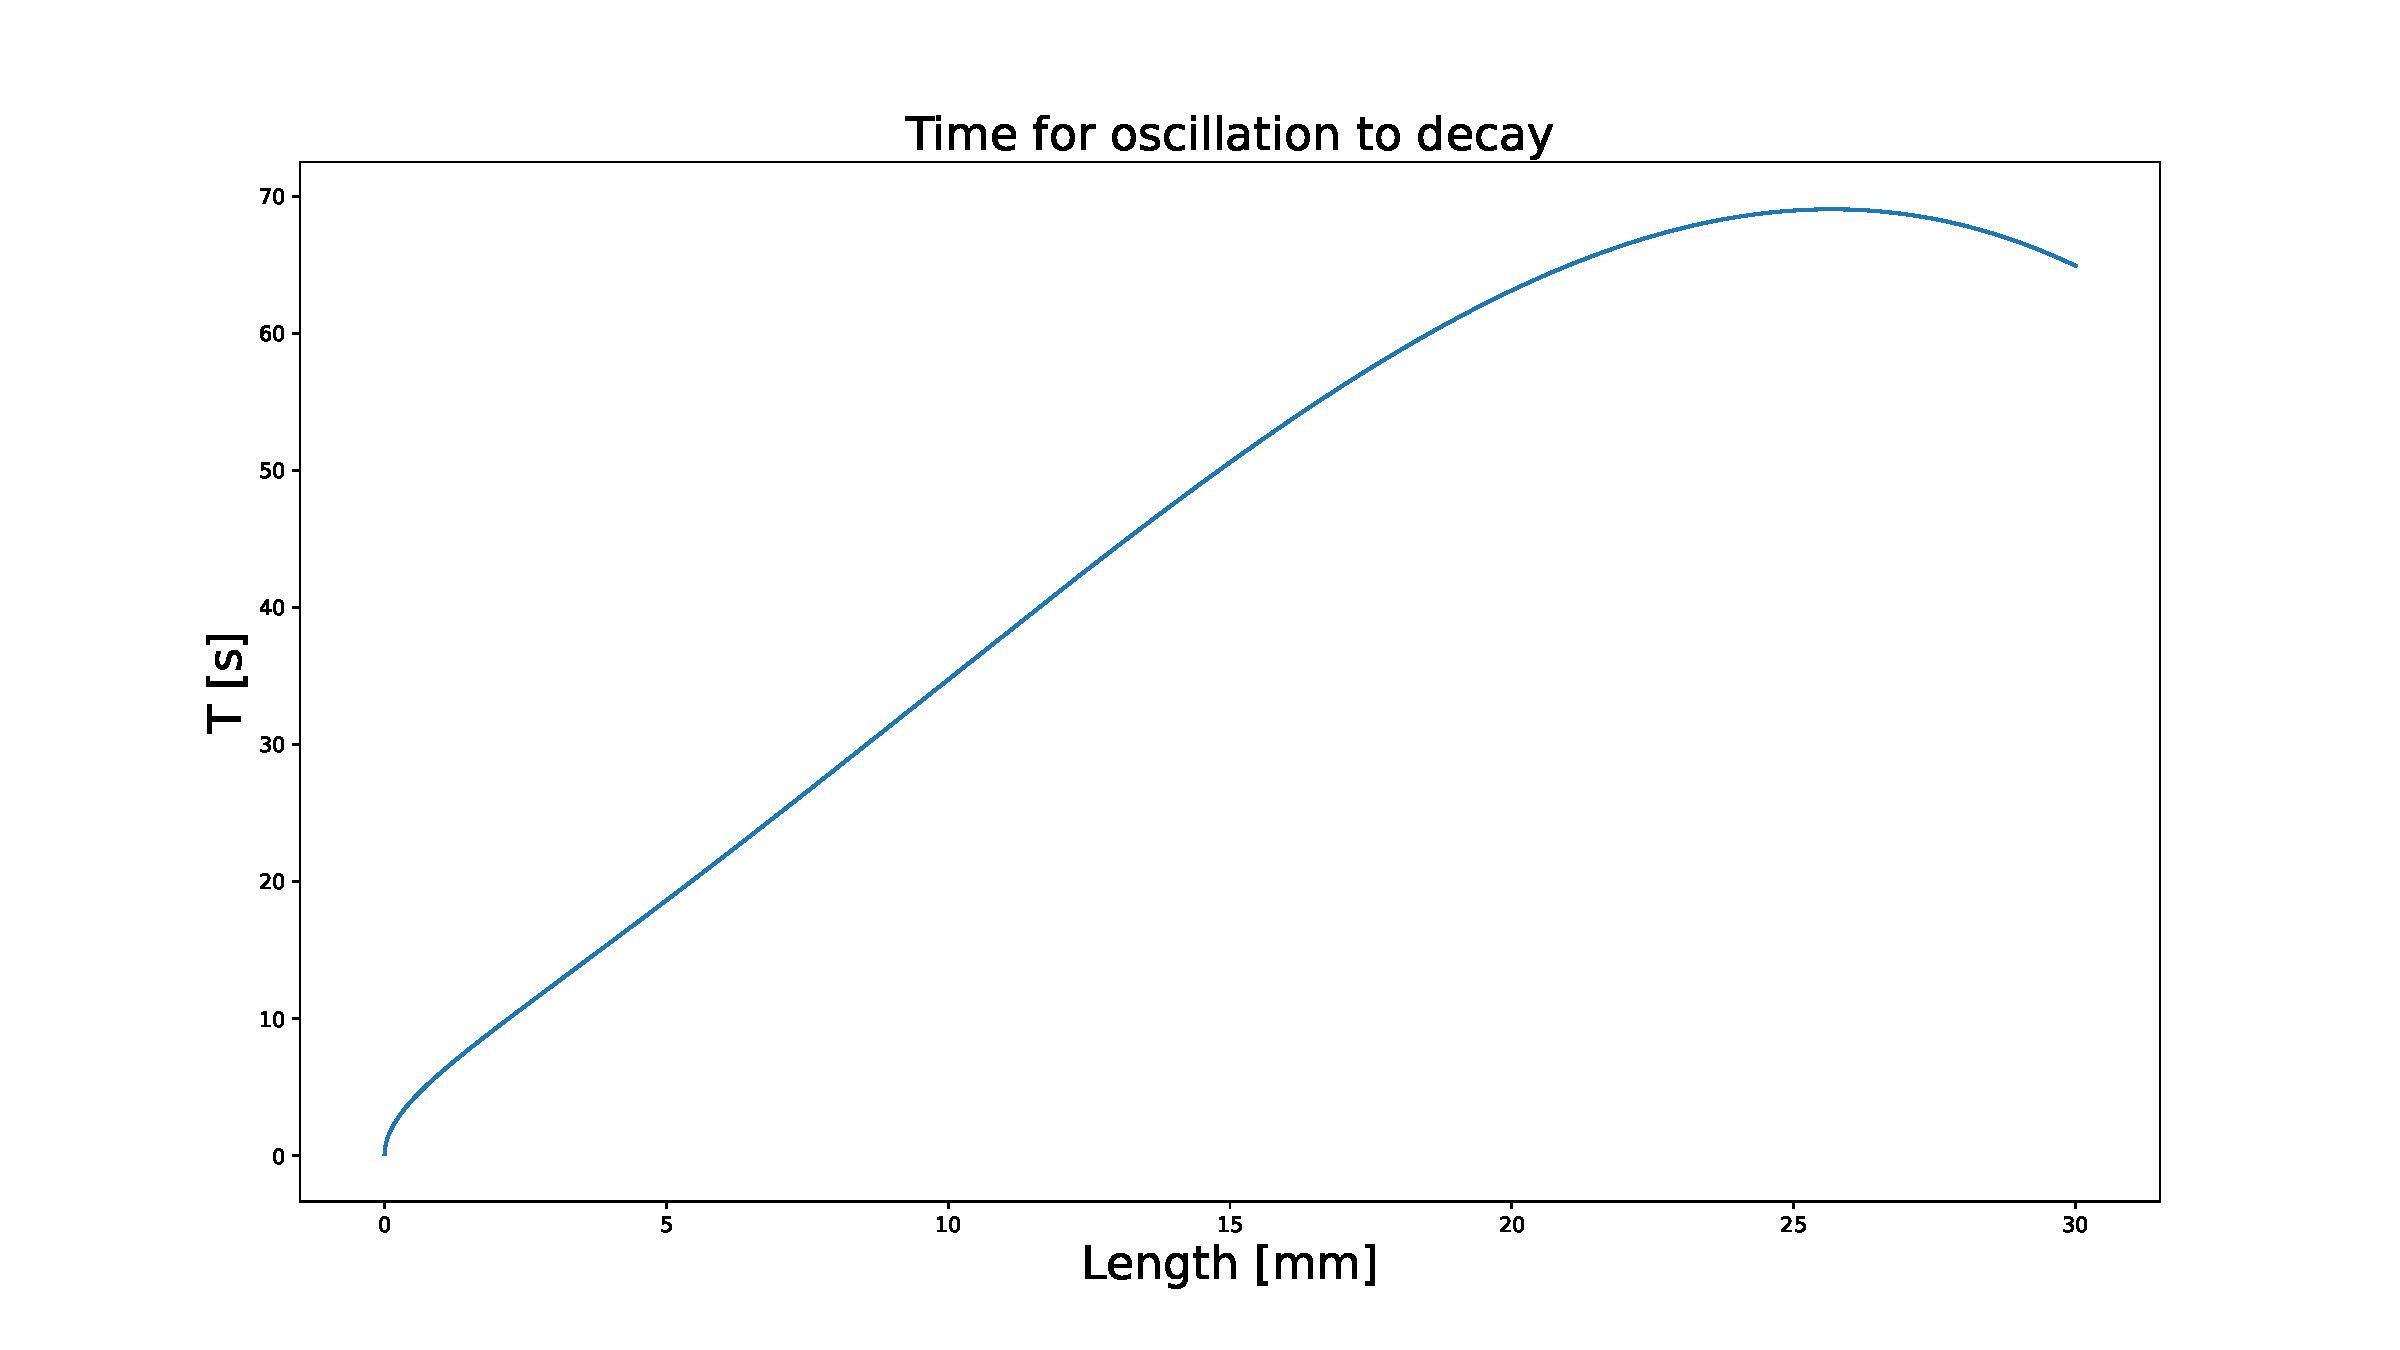
\includegraphics[width = \textwidth]{figs/2.d.pdf}
  \caption{Plot av tid for lyden å dempes}
  \label{fig: 2.d}
\end{figure}
\end{enumerate}

\subsection*{Oppgave 3}
\begin{enumerate}[a)]
\item
Vi har
\[
\frac{\mathrm{d}^{2} Q}{\mathrm{d}t} +  \frac{R}{L} \frac{\mathrm{d}Q}{\mathrm{d}t} + \frac{1}{CL} = V_0 \cos \left(ω_ft\right) 
\]
Ettersom ligningen er helt analog med likningen for en harmonisk svinging kan vi bruke ligningene fra tidligere til å finne verdiene i ligningen. 
\[
\ddot{x} + \frac{b}{m} \dot{x} + \underbrace{\frac{k}{m}}_{ω_0} x = \frac{F}{m} \cos \left(ω_ft\right) 
\]
\[
\frac{b}{m} = \frac{R}{L} \quad , \quad ω_0^2 = \frac{1}{L C} \quad , \quad \frac{F}{m} = \frac{V_0}{L} \quad , \quad \frac{k}{m} = \frac{1}{LC} \quad , \quad m = L 
\]
\[
k = \frac{1}{C} \quad , \quad b = R \quad , \quad  F = V_0 \quad , \quad ω_0 = ω_f
\]
Faseskiftet er gitt ved 
\[
\cot ϕ = \frac{m(ω_0^2 - ω_f^2)}{ω_f b} = \frac{\frac{1}{L C} - ω_f^2}{ω_f R / L}
\]
Amplituden er gitt ved
\[
A = \frac{F / L}{\sqrt{(ω_0^2 - ω_f^2)^2 + (ω_f R / V_0)^2}}
\]
Q-verdi er gitt ved 
\[
Q = \sqrt{\frac{mk}{b^2}} = \sqrt{\frac{L}{R^2C}}
\]
Amplituderesonansfrekvens er gitt ved
\[
f_{\text{A. res}} = \frac{1}{2 \pi} \sqrt{ω_0^2 - \frac{b^2}{4m^2}} = \frac{1}{2 \pi} \sqrt{\frac{1}{LC} - \frac{R^2}{4L^2}}
\]
Faseresonansfrekvens er gitt ved
\[
f_{ϕ_{\text{res}}} = \frac{1}{2 \pi} ω_0 = \frac{1}{2πLC}
\]
\item 
Vi finner Q-verdien til kretsen ved å bruke verdiene oppgitt. 
\[
Q = \sqrt{\frac{L}{R^2C}} = \sqrt{\frac{25 ⋅ 10^{-6}}{1^2 ⋅  100 ⋅ 10^{-9}}} = 15.81
\]
\end{enumerate}
\end{document}